\chapter{Implementation}

\section{User interface}
\label{mainimp}
The main display represents the general interface is displayed to the user. This is where the algorithms visual representation will be presented, as well as providing the location of the user interaction elements enabling modification of the algorithms parameters. This interface is a result of the contents of the DisplayFrame Class and its contents. The design for this view is almost as described in section \ref{ssec:mainUI}, appendix B, however, there has been a slight modification to this proposed design.

\begin{figure}[H]
\centering
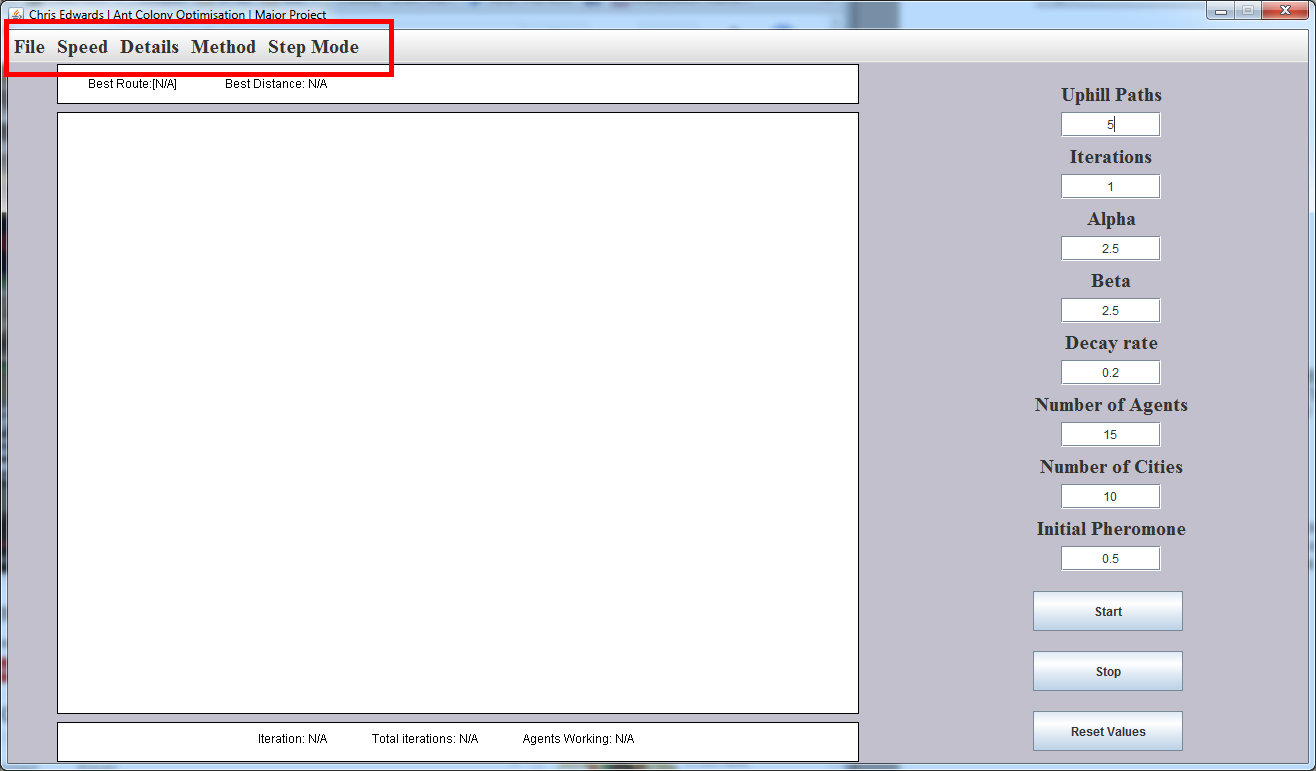
\includegraphics[scale=0.35]{Images/chapter4/displayFrame}
\caption{Implementation of the proposed user interface. The contents of the red polygon highlights the additional features not present in the initial design.}
\label{fig:displayFrameImp}
\end{figure}

The additional features highlighted by the red polygon in figure \ref{fig:displayFrameImp} represent the features which were not initially designed. These features are represented in a separate location to the control panel (right hand side of figure \ref{fig:displayFrameImp}) as there is no logical connection between the menu bar features, and the modification of the algorithm parameters. The author opted to use a menu bar to control the access to these features as the vast majority of users will recognise what a menu bar is, and understand how to interact with such elements. 

The different elements contained in this menu bar relate to general system interactions. The File option enables the user to either load, or save a configuration to a specified file. The Speed option enables the user to change the Thread speed, which will directly change the algorithms rate of execution. The Details menu is used to control access to any additional views. The views which can be access here are; the Uphill Viewer (section \ref{uphillview}), The City Detail View (section \ref{deetzlview}) and the Equation Viewer (section \ref{eqnlview}). In addition to the access of these extra views, the Detail menu also enables the user to disable and enable uphill routes \Large REFERENCE UPHILL ROUTES GENERATION ALGORITHM PSEUDO CODE \normalsize to be generated for current problem. The Method option enables the user to select the current algorithm type from a list of implement algorithm types. Currently the author has implemented a Basic Ant System and an Elitist Ant system so the user can switch between these algorithm types. The Step Mode menu enables the user to enable or disable the step mode functionality. When enabled, step mode will allow the user to step through the algorithms execution at their own pace without the application automatically solving the problem.

\section{Data Structures}

\subsection{Pheromone and Distance Matracies}

\subsubsection{Pheromone}
\label{phero:struct}
A Pheromone Object is used to represent the pheromone concentration for a given edge in the current problem graph, however there is no data stored inside the Pheromone Object which relates this Object to a specific edge. To enable logical indexing of these Objects such that the author could continually the pheromone data for a specific edge is a fairly trivial task however, the method of doing so has changed since the initial proposed design as seen in section \ref{pheroRepsec}, appendix B.

The concept of a using two-dimensional array to store the pheromone data is still present however, the dimensions of such structure are now directly representational of the number of cities present in the current problem. Assume there are $x$ number of cities in the current problem then the length of each array would also become $x$. Therefore the instantiation of the pheromone data structure is of the format $Pheromone[][] pheromone = new Pheromone[x][x]$. Assuming these $x$ cities have the $index$ values $0, 1, ..., x-1, x$ then indexing any edge would be done using the format $pheromone[x][y]$. Given this format, $x$ and $y$ are any valid $City indexes$. For example, to access the pheromone concentration for the edge corresponding to the path from $City\ 0$ to $City\ 5$ would be accessed using $pheromone[0][5]$. As accessing an element in in an array is a $O(1)$ operation this method of access is extremely efficient and supports a problem of almost any size as the data structure resizes with the problem. Figure \ref{initPheroCode}, appendix C represents how the pheromone matrix is initialised using the initial pheromone value for all edges.

\subsubsection{Distance Matrices}

Initially there was no proposed design for the inclusion of data structures representing the distances between each node in the graph as the initial design for the problem representation made it simple to calculate the distance between the current node and the destination node extremely trivial. The author decided that as the problem representation has changed to the TSP there needs to be a better method of accessing the distances between two nodes (Cities).

The design for the distance matrices are based on the implementation provided by Thomas Jungblut \cite{tjung:aco:blog}. The implementation of these data structures is identical to that discussed in section \ref{phero:struct} however, the data stored in each array element represents the $euclideanDistance$ between two $cities$ rather than the pheromone concentration. As defined in section \ref{phero:struct} the size of distance matrices will represent the number of cities. If there are $x$ cities in the current problem then the format for instantiation will be $double[][] distanceMatrix = new double[x][x]$. The way in which elements are accessed also remains the same as above, however once instantiated these values will remain constant as a $City$ cannot move location. These matrices are easily populated after the cities have been instantiated. The code in appendix C figure \ref{initDistanceCode} represents how this has been implemented. A correct implementation would return a distance of $0.0$ if $index[x][x]$ were to be accessed where $x$ is the same value. This is because the distance from any $City$ to itself is 0.
As the probability is represented as $p_{xy}^{k} = \frac{(\tau_{xy}^{\alpha })(\eta _{xy}^{\beta })}{\sum (\tau_{xy}^{\alpha })(\eta _{xy}^{\beta })}$ where $\eta _{xy}$ represents $\frac{1}{distanceMatrix[x][y]}$ (inverted distance). As this function is used extremely often during the algorithms execution rather than converting the value of $distanceMatrix[x][y]$ every time an inverted value is needed it is far more efficient to store an inverted version of the $distanceMatrix$. The code snippet in figure \ref{initInverteddistanceCode} demonstrates how this can be implemented. The $invertDouble(distanceMatrix[i][j])$ in said figure simply returns the value of $\frac{1}{distanceMatrix[i][j]}$ however if $distanceMatrix[i][j]\ ==\ 0.0$ then $0.0$ is returned as $\frac{0.0}{distanceMatrix[i][j]}$ is illegal.
  
\subsection{Agent and City Collections}

Both Agent and City Objects are designed to be stored using data structures which implement the List$<$type$>$ Java interface. As the number of Cities and Agents present in the current problem is dynamic and user defined the size of the data structure must be established at runtime and therefore the data structure chosen must scale well and maintain performance regardless of its size. In addition to this, a user is able to modify the amount of Agents and Cties once created, therefore the data structure must be able to be effectively resized dynamically without complication. The ArrayList data structure has been chose to store the Agents and Cities as it is scalable and can be dynamically resized. An Array implementation could be used here however, if the Array reached capacity then there would need to be conditionals put in place by the author to copy the contents of the full Array into a new, larger Array instance. The use of ArrayList means that the author does not have to worry about these conditionals are they are handled for the author by the ArrayList implementation. In addition to this, the order the elements in generally unimportant, accessing a random index however is. Using an ArrayList provides $O(1)$ random element access using the provided $get(index)$ method. Also inserting into an ArrayList is $O(1)$ where as an Array implementation would provide $O(n)$ insertion as the next free index would have to be located. As the ordering in unimportant there is no reason to use a LinkedList data structure and the improved performance of the ArrayList versus an Array has enabled the author to confidently select an ArrayList implementation as the best suited data structure. 

Unless explicitly stated by loading a configuration from a file, the locations of the $City$ elements in collection of cities are randomised. There are conditionals in place to ensure that two cities cannot be placed in the same location as this is a possibility if the locations of such cities is random. The implementation of the $City$ instantiation can be found in appendix C, figure \ref{initCity}.

The starting location of the Ant Objects represented as elements in the collection of agents is also randomised. This random value is however limited to a range of integers with a maximum possible value equal to $cities.size() - 1$. As indexes start at 0, this enables the random function to return any $City$ index such that it is possible for an agent to start at any $City$ location. The implementation of this agent instantiation is defined in appendix C, figure \ref{initAnt}.

\subsection{Best Route representation}
\label{bestrtoutey}
Storing the current best route is slightly more complicated than storing the collection of Agents or Cities as the ordering is important. As the ordering is important the accessing of random indexes is irrelevant as the elements stored in this data structure when parsed in order represent the order to cities which the agent visited in order to produce this best route. The indexing of random elements would enable the elements to be parsed in an incorrect order, thus this functionality will not be used by the author and therefore the data structures performance in executing such task is completely nullified. The data structure used for this representation does not need to have dynamic resizing capabilities as the length of any best route will represent the number of cities in the problem as an agent must visit every City once and only once. The author reduced his choice to using an ArrayList or a LinkedList implementation. A LinkedList implementation has massive performance enhancements when compated to an ArrayList as a LinkedList can provide constant time ($O(1)$) insertion and deletion operations using iterators which can be relied upon regardless of the magnitude of such data structure in combination with the lack of regard to element ordering. An ArrayList cannot reliably provide such performance. This in addition to the fact that the ordering of elements is important, has lead the author to decide on using a LinkedList data structure for the representation of the best routes.

\section{Pheromone Operations}

The translation of the pseudo-code described in algorithm \ref{aco:pseudo:pherofunc} was a fairly simple process as the pheromone algorithm is itself relatively simple. Once implemented the author quickly realised that the pheromone operations (deposit and decay) were not behaving correctly. During the course of agents $move()$ method every time the agent moves from its current location to its next location pheromone proportional the distance travelled would be deposited on the corresponding edge. The problem was that every time this pheromone was deposited the global pheromone was in fact being decayed so the global pheromone was being decayed every time the agent moved. In order to prevent this problem from arising rather than directly updating the pheromone on the edge when the ant moves the agents pheromone deposit on this edge is instead added to a secondary $newPhero$ variable in the Pheromone Object for this corresponding edge. This variable is used to collate the total amount of new pheromone to be deposited for any edge. When it is time to update the edge pheromone, every Pheromone Object is iterated through and value present in this $newPhero$ variable is used in the pheromone calculation allowing for correct behaviours to be represented. This is slightly more complicated than the author envisioned however, the additional complexity is essential to ensure correct behaviour. The implementation of this method is shown in appendix C, figure \ref{codephero}.

\section{Solving the Problem}

The author encountered unforeseen complications when implementing the pseudo-code represented in algorithm \ref{aco:pseudo2}. The subsections below described the problems with the implementation process and their associated solutions.

\subsection{Agent Movement}
\label{antyMove}
The author has problems initially with his implementation of the probability based movement of the agents. The implementation of the Ant's $move()$ function worked as expected there were no complications associated with that however, the complications that the author encountered involved the probabilistic selection of the Ant's next location. The problem caused every Ant that started at the same City index to take exactly the same route. Upon debugging the Ants $getNextProbableNode(int\ y)$ function the author realised that there was in fact no random element associated with this method and the City with the highest probability was constantly selected thus, the Ants never had the ability to divert away from the best looking route causing local solutions to be present. The author attempted to implement this random element into his method however the algorithm did not perform as efficiently as expected. Thomas Jungblut had provided an open source implementation of a basic Ant Colony Optimisation algorithm \cite{tjung:aco:blog}. This implementation was provided free of charge and allowed modification which enabled the author to replace his lacklustre node selection function with the one provided in this working implementation. This node selection function did however require modification by the author to ensure correct operation with his architecture. Once this method had been modified and implemented the node selection process for the Ant's next location worked as initially intended. The author realised that his implementation took completely the wrong approach which involved sorted the candidates locations based on their associated probability. Had the author not accepted that the re-use of a working implementation is the best way to progress the application then a reduction in project quality would have been a possibility. The implementation of this node selection method can be seen in appendix C, figure \ref{nextNodeCode}. If this method returns $-1$ then the Ant is deemed to have completed its walk.

\subsection{Automated Solving}
\label{autoSolve}
Implementing an algorithm which once started, executes until completion was in fact fairly simple to do initially. This simplistic implementation stemmed from the fact that initially the algorithm only considered the fact there was one iteration. As there was one interaction it was simple to define a stop condition which was in fact when every agent had completed its walk which meant the algorithm stopped when $Ant.getFinished()\ returned\ true$ for every Ant. Once the author had implemented automatic execution for one interaction, the ability for a user defined number of interactions was implemented. The addition of to support $x$ number of iterations where $x\ >\ 1$ introduced several new complications. Each new iteration meant that the Ants need to be reset so that they forget everything from the previous iteration(s) but the pheromone levels, Cities and current best route must all be persevered across iterations. In order for this to be possible, the author adapted to algorithms stop condition to now be relative to the number of iterations or in other words stop when $currentIteration\ ==\ totalIterations$. A new iteration is started when all Ant's have finished their walk, instead of checking every Ant for the condition $Ant.getFinished()\ ==\ true$ once an ant had finished a variable representing the total number of Ants current working (unfinished) was reduced by 1. When this value reaches 0, there are no Ants currently working thus the iteration has completed. Once an iteration has completed the Ants must be reset so the next iteration can start, this is done by calling the $initAnts()$ method again on the current $World$ enabling the old Ants to effectively be reset. The variable representing the number of Ants working is also reset so that $antsWorking\ ==\ totalAnts$ and the process starts again. During this reset operation the pheromone levels, cities and best route remained unchanged to ensure previous iteration results remain. The implementation for this algorithm can found in appendix C, figure \ref{iterationThing}.

\subsection{Step Based Iteration}

In order to implement an algorithm which executes on a step-by-step basic will require constant user interaction in order to execute to completion. In order to achieve this, several modifications have been made to the algorithms used in the process of automated solving. The first problem associated with step based iteration is the fact that an Ant must be stopped moving after it has moved to its next location, in comparison the fully automated approach uses an algorithm which ensures an Ant continues moving until it is finished or move while the algorithm in figure \ref{nextNodeCode} does not return $-1$. In order to stop the Ant after one movement the algorithm in section \ref{antyMove} can remain largely the same, however this while loops must be removed so that the movement function executes once and only once per step. This change alone however is not enough to stop the algorithm from executing until completion. Rather than using a $for\ each$ loop to iterate through every Ant and instructing it to move as described in figure \ref{iterationThing} there must now be a way to track the current Ant which is moving and update this tracker once said Ant is finished. In order to do this an index representing the location of current working Ant is stored so that when the algorithm is stepped through only the Ant and that index is signalled to move 1 step. Once this Ant has finished, then this index is incremented until $index\ >=\ agentsCollection.size()$. Similar to the algorithm described in section \ref{autoSolve} once every Ant has finished walking, the iteration is complete and if there are more iterations to execute then the Ants and index are reset. Although this feature wasn’t part of the initial or improved design, the ability to re-use the existing algorithm enabled the implementation of the feature to be far less complex. The implementation of this step based iteration can be seen in figure \ref{stepM8}.

\section{Rendering the Algorithm}

The implementation of the pseudo-code represented in algorithm \ref{aco:renderPesudo} turned out to be far more complicated than the author actually planned. The subsections below segment the complications that arose and the steps the author took in order to ensure a proper visualisation process.

\subsection{Swing Worker}
\label{swingmeupm8}
Initially the algorithm was executed on the AWT event-dispatching thread. The automated solving algorithm is a fairly long and somewhat resource intensive process and given that the graphical user interface elements are also executed on this thread. This causes problems during execution. During the algorithms execution time as the interface and algorithm are both on the same thread, the user interface would freeze and become unresponsive until the algorithm had completed. The implication of this are that literally none of the algorithms execution is visualised, which is the complete opposite of the intended implementation. The author realised that this is extremely bad design and in order to correct such complications concurrency should be introduced into the system. The graphical user interface is built up of several Swing component and these components are not thread safe which can cause some concurrency problems. As a result of these components not being thread safe the Java language is defined such that any access to these components must be done from within the same thread which happens to be the Event Dispatch Thread. In order to both modify the user interface and execute the algorithm in a concurrent manner the author has used the $SwingWorker$ Object provided by the Java language specification. A $SwingWorker$ is designed to perform length tasks which interact with a graphical user interface adhering to the language specification protocols. The $SwingWorker$ has a $doInBackground()$ method which executes this method inside a separate $Worker$ thread. During the execution of the $doInBackground()$ method any interactions with the Swing components are dispatched on the correct Event Dispatch Thread by the $SwingWorker$. As a result the author has been able to implement concurrency to allow for the parallel execution of the algorithm and interface modification relatively complication free. The code contained within this applications $SwingWorker$ is shown in figure \ref{iterationThing} and is the location of the algorithm discussed in section \ref{autoSolve}. 

The step-based iteration method of solving does not need to worry about such complications as each step takes very little time to complete, thus the addition of a $SwingWorker$ to facilitate such behaviour is over complicating the situation and will not benefit the user in any way.

\subsection{Visualising Agent Movement}
\label{visy}
One of the major problems associated with the visualisation of the algorithms execution is accurately representing the agent’s movement between two cities. Initially the agents would move between cities without any indication to the user about which path the agent took as the agents themselves would seem to teleport from one city to the next. This is not the kind of feature that should be present in an application of this kind. The author decided that there needed to be a way to visualise the Ant’s movement between cities however, the visualisation of this movement should be simple so that it doesn’t over complicate a simple action such as moving from one point to another. Given that every $Ant$ stores the indexes of the last two cities it visited in a variable $movementTracker$. This variable is an array of integer values of size 2 and it will only ever contain the last 2 cities the agent visited, thus $movementTracker[0]$ represents where the Ant started prior to moving and $movementTracker[1]$ is where the Ant finished.

The author decided that as the coordinates of the two cities stored in this $movementTracker$ variable are fairly simple to obtain it would be straight forward to use linear interpolation to draw a visual aid along the Ant's movement path in order to highlight which path the Ant took. Given a start and end coordinates for a line Linear Interpolation can be used to find the coordinates for any point along that line. 

\begin{figure}[H]
\centering
\begin{gather*}
\Huge
result_x\ =\ x_1\ X\ (1\ -\ \mu)\ +\ x_2\ X\ \mu \\
result_y\ =\ y_1\ X\ (1\ -\ \mu)\ +\ y_2\ X\ \mu
\end{gather*}
\caption{Formula for Linear Interpolation where $x_1,y_1$ are the start coordinates, $x_2, y_2$ are the end coordinates and $\mu$ is the location to find \cite{interpolation:site}.}
\label{fig:interPolateEqn}
\end{figure}

Once the coordinates of the two cities stored by index in the $movementTracker$ variable have been retrieved they can be passed to the $LinearInterpolateX(double\ x1, double\ x2, double\ mu)$ and $LinearInterpolateY(double\ y1, double\ y2, double\ mu)$ methods in order to find a point on the line between these two City locations, this line is representive of the path the Ant will take to travel between said locations. The correct $\mu$ value must be selected in order to provide the best representation. The author opted to go for drawing a series highly visible ellipsis along the line with the distance between said ellipsis to be 0.2 which is the equivalent to approximately 20\% of the lines total length. These ellipsis will therefore be drawn using rhe retuned values from the equantions in figure \ref{fig:interPolateEqn} where $\mu\ = 0.2,\ 0.4,\ 0.6,\ 0.8$. This will enable the user to clearly identify which path has been taken and also enable the user to judge the length of said path as the longer the path the greater the spacing between the ellipsis. The code implementation of the equations in figure \ref{fig:interPolateEqn} is shown in figure \ref{linearCode} and the code for drawing the path the Ant takes is shown in figure \ref{antWalk}.

\subsection{Scaling}
\label{scaley}
In order for the visual representation to be rendered in a suitable manner there has to be some form of scaling to ensure all the visual elements remain in aspect to each other. The size of the canvas area is fairly limited so the author had to decide on a scale factor which enabled the complete representation to be container within the canvas bounds. The author decided that as the canvas area is $800px$ in width and $600px$ in height a scale factor of 20 is perfectly suited to this environment. As 20 is a factor of both 800 and 600, this will effectively provide the author with a grid for 20 x 20 squares which is 40 x 30 in dimension. If a scale factor greater or less than 20 were to be used then the dimensions of this grid would change and if this scale factor was too large there would not be enough room to display an adequate amount of detail. There are also complications with using a scale factor which is too small, this will cause the visual elements to be difficult to see as they will appear very small on the canvas which may alienate some users.

This scale factor will be applied when rendering any element on the canvas which includes the rendering of City locations, Agent locations and drawing paths between cities. If a City has the $(x,y)$ coordinates of $(18, 15)$ and the author used no scale factor to scale this when rendering then the City would be rendered at $(18px,15px)$. If a further two cities had the $(x,y)$ coordinates of $(30, 5)$ and $(2, 9)$ respectively with no scaling applied these cities would be rendered extremely close to each other which would make it difficult to visualise the algorithm execution as the world would occupy an extremely small amount of canvas real estate. Applying this scaling factor to same set of cities and coordinates causes the cities to be rendered at $(360px,\ 300px), (600px,\ 100px)$ and $(40px,\ 180px)$. This produces a world where the cities are suitably spaced such that there is sufficient room to render the algorithms execution and visualise the Agents movements between such cities. This scaling factor is hidden from the users. As far as the user is concerned when creating a file for use in loading a problem configuration a cities $(x,y)$ location is specified in terms of its grid square location rather than in terms of scaled coordinates as shown in section \ref{fileIO}.

\subsection{Painting the Canvas}

Every aspect discussed in the section is vital in the painting of the algorithms execution for the reasons stated above. As every aspect of the algorithm needs to be visually represented the actual painting of the algorithm to the canvas became more complex than the author initially envisioned. 

Representing the City locations cities is fairly simple to implement as every City stores the location for its $(x,y)$ coordinates. In order to render each City at its correct location, the collection of cities is iterated through and the method $drawOval(City.X X 20,\ City.Y X 20, 20, 20 )$ is used to draw an oval which has the width and height of $20px$ and is represented in the correctly scaled location. There is a slight problem with this implementation however. As discussed in section \ref{scaley} the canvas is segmented in a grid 40 x 30 in dimension therefore the coordinates representing a grid cell represent the top right corner of such cell. If a City is drawn at $(20,10)$ then this will be drawn in the top right corner of the grid square $(20,10)$. The author found this to be visually off putting and didn’t produce the look the author wanted. In order to prevent this the location of the drawn city must be offset such that rather than being drawn in the top left of grid location it is then drawn in the centre of such grid location. In order to do this a simple change to the $drawOval$ is methods parameters is required. The modified version of this method call now resembles $drawOval((City.X * 20) - 10,\ (City.Y * 20) - 10, 20, 20 )$ where 10 represents $\frac{scaleFactor}{2}$ this will now draw the cities centred into the correct grid square. These cordinates are also used to render the ants at a city location. As every Ant stores the index of the City it is current at, it becomes trivial to found the locaton where it should be drawn by iterating through the collection of cities untill the index is found.

Representing the path between these cities is also a somewhat simple task. These routes are used to visually display the routes which any agent can take to navigate between any two cities. As the graph is being represented as a fully connect graph where any City can be reached from any other City, the paths displayed to the user must reflect this. Each path will be displayed as defined in section \ref{visy} which is as a line drawn from one City to another. The collection of cities will be iterated through, and for each City in the collection the collection of cities will be iterated through again. The first iteration of the collection will represent the start location for each line (path) then whilst keeping this location the same, the next iteration of the collection will be used as the end location for the line (path). This is a simple way to draw a line from each City to every other City.

As these lines represent the paths between cities, they are therefore used to represent the edges connecting nodes (cities) in the graph and as a result these lines are also to be utilised for the visualising of the pheromone concentrations on such edges. In order to represent the pheromone the author has decided that the opacity will change in proportion to the pheromone concentration on their given edge. As the pheromone values for a given edge can become incredibly small ($<<\ 0$) depending on the number of iterations, cities and agents the opacity of such lines must be based on a suitably scaled version of the pheromone values on each edge. The author decided use a scale factor of 2000 when applying the pheromone concentration to the opacity of the corresponding line however, the opacity (alpha) level for a given line is an 8-bit integer thus 255 is the maximum value. To prevent conversions of $pheromoneConcentration_{xy}\ X\ 2000\ >\ 255$ causing problems there is a condition to catch larger values and reduce their size to maximum legal value of 255. As the pheromone concentration gets lower and lower the paths with start to become invisible to the user so they can easily see which paths are actually being used.

Displaying the best route to the user is the most complex part of the visualisation process and also one of the most important. The implementation of this feature was far more complex that the author expected and its complexity extends further than simply drawing a red line. As a line requires a start and end location this means that the best route data structure (see section \ref{bestrtoutey} must be iterated in pairs, and accessing these pairs is not as elegant as the author has planned. The best route will be created using a series of lines drawn between such pairs. Once the first city of such pair has been identified the next element in the data structure is the second City belonging to the pair however, the author first has to check if there is infact a next element before such an action can take place which is simply doing using a condition similar to $(elementIndex + 1)\ <\ bestRoute.size()$. If this condition returns true then continue with the line drawing process as there is a valid pair of cities to draw a line between. Once this pair of cities have been identified it is simple to draw a line between them as the coordinates are known. The complexity comes from the multiple iterations of the City collection in order to locate the City pairing, this makes the code block slightly more difficulty to both debug and mentally visualise which made this feature slightly harder to implement. The code for such a feature is shown in figure \ref{bestCode}.

\section{Elitist Ants}

The addition of Elitist Ants was slightly more complex than the author initially thought however, as a whole it is not an overly complex feature. The algorithm remains largely unchanged from the Basic Ant System, the added complexity comes from the fact that pheromone needs to be deposited on the Elite Ant best routes every iteration. Correctly storing and updating the current $x$ number of Elite Ants was simple to implement for the author and involved checking to see if this agent should be an Elite Ant or based on its total distance travelled. The implementation for this is shown in algorithm \ref{aco:pseudoEAS}, lines 19 to 24 as remains as designed. As discussed with the rendering of the best route, the deposit of pheromone along can be done so using a pair based iteration. This is slightly less complex that the rendering process as there is no need to retrieve the City coordinates, As the pheromone matrix is set up in a manner such as that stated in section \ref{phero:struct} only the City indexes are needed. Once a pair of City indexes has been extracted from the best route pheromone can be deposited along the route in a fashion similar to this $pheromone[CityPair1.index][CityPair2.index].addToNewPheromone(pheromone$ \\ $[CityPair1.index][CityPair2.index].getPheromone\ +\ e )$ where $e$ is a constant representing $\# \ of-$ $cities$. The code for depositing pheromone of the $x$ number of elite routes is shown in figure \ref{elitePhero}.

\section{Uphill Path Generation}

The implementation of uphill paths was itself fairly simplistic and involves the process of locating the route's corresponding element in the distanceMatrix and doubling the value contained in such element. This enables an uphill path to effectively cost double its normal cost. Depending on the current $\beta$ value, the agents will generally have a higher probability of taking a shorter path. As this is the case the addition of such uphill paths allows the algorithm to potentially produce a wider range of solutions to the same problem configuration.

The selection of these uphill routes is slightly more complex than the author assumed them to be. The location of these uphill paths is randomly generated. The location is determined by using the $Random.nextInt(\#\ of\ cities)$ method to randomly select an element from the distance matrix. This element represents an edge length between two cities, thus doubling this value will effectively double the distance between said cities making this edge cost more to traverse than usual. There are problems with using a random selection process for selecting the start and end locations for this uphill path however. These start and end locations will be valid city indexes which means that these two randomly generated values cannot be the same as there is no edge from a City to itself. This is where the added complexity is introduced. The author must now check that the randomly generated values are in fact different, if they are equal then the random generation process must happen again. As the random value generated is in the range of $0...cities.size()$ how likelihood of these random values being the same is dependent on the magnitude of the value range. If there are few cities then this random generation process make have to be executed an inefficient number of times until two non-identical values are generated, this is not really a problem if there are a large number of cities. The code representation for the generation of uphill routes is shown in figure \ref{suchUphill}.
